\documentclass[10pt]{article}
\usepackage[utf8]{inputenc}
\usepackage[T1]{fontenc}
\usepackage{graphicx}
\usepackage[export]{adjustbox}
\graphicspath{ {./images/} }
\usepackage{amsmath}
\usepackage{amsfonts}
\usepackage{amssymb}
\usepackage{mhchem}
\usepackage{stmaryrd}
\usepackage{bbold}

\title{Jinchao Xu }


\author{Deep Learning Algorithms and\\
Analysis}
\date{}


\begin{document}
\maketitle

Summer 2020

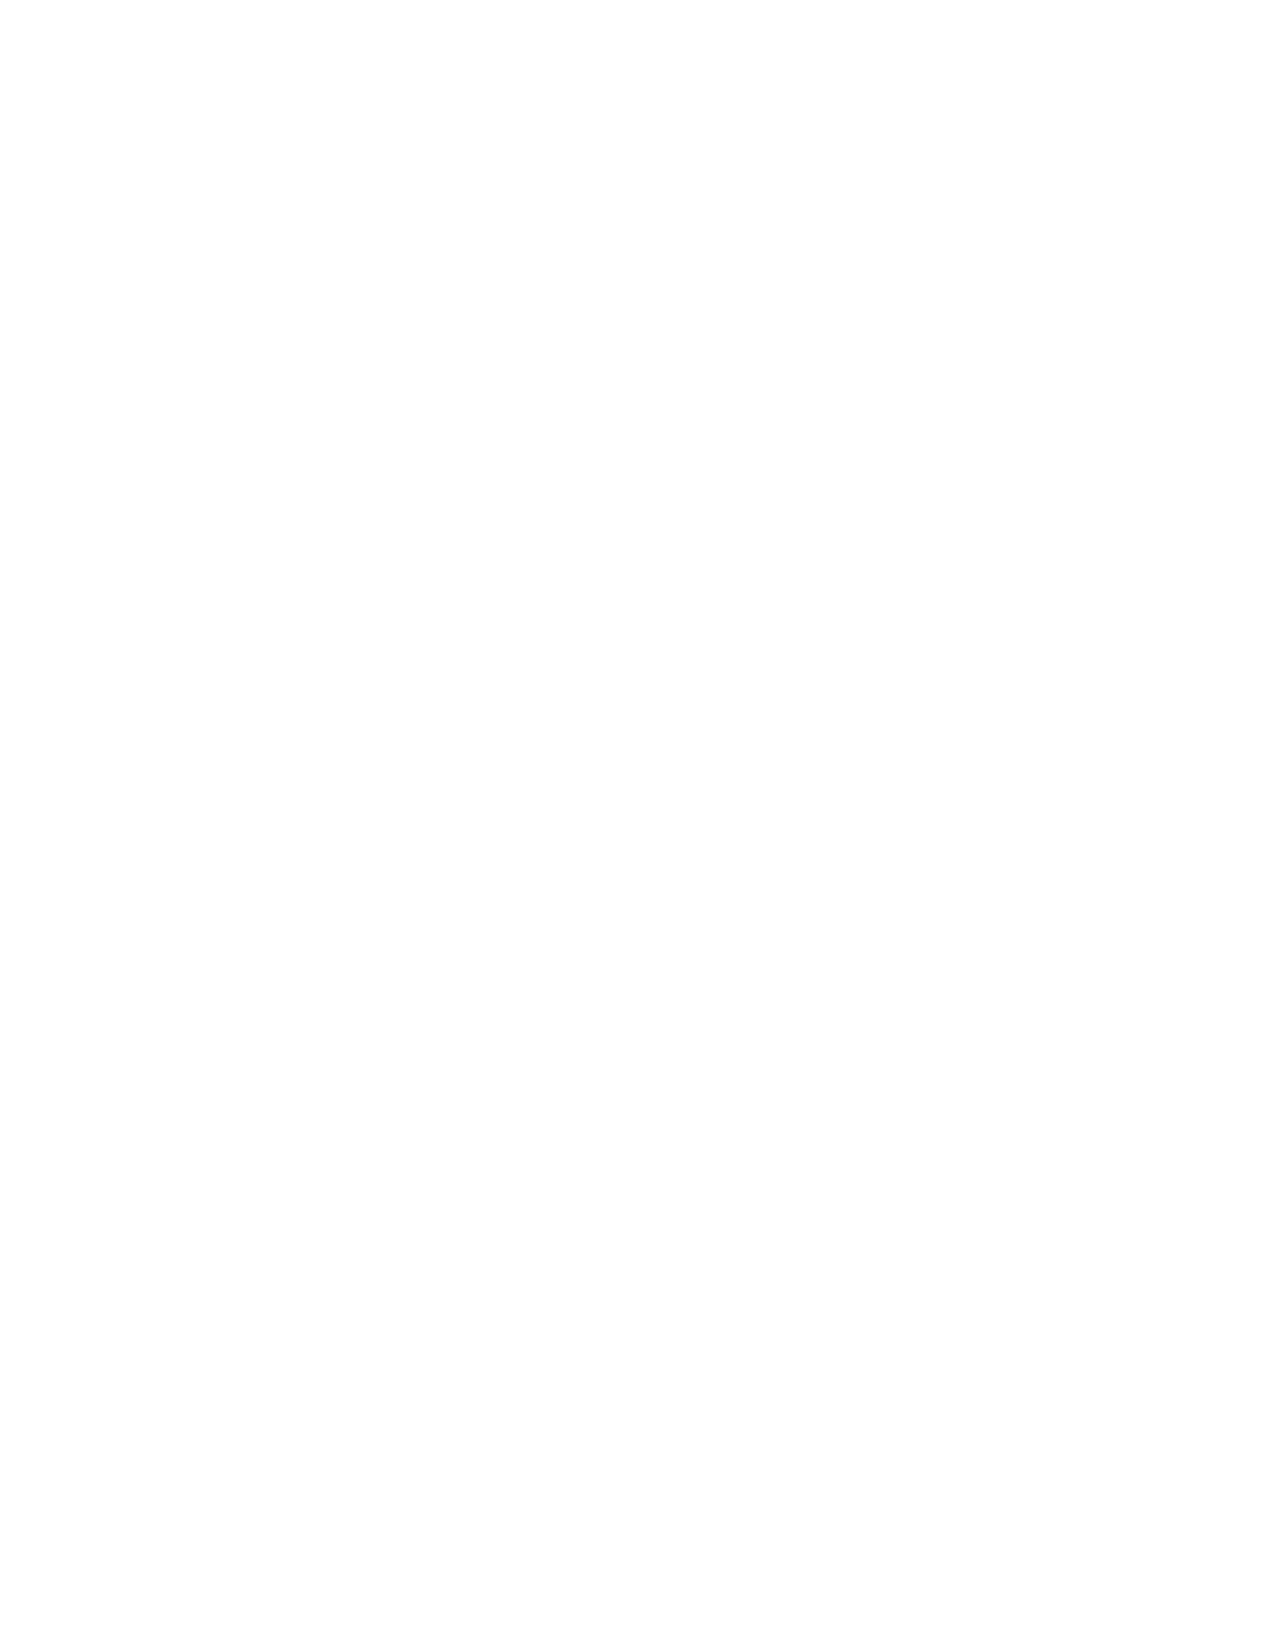
\includegraphics[max width=\textwidth]{2022_01_05_20c4aca6821d56656c19g-2}

\section{Contents}
$1 \quad$ Nonlinear Models $\ldots \ldots \ldots \ldots \ldots \ldots \ldots \ldots \ldots$

1.1 Nonlinear classifiable sets $\ldots \ldots \ldots \ldots \ldots \ldots \ldots \ldots \ldots$

References $\ldots \ldots \ldots \ldots \ldots \ldots \ldots \ldots \ldots \ldots \ldots \ldots \ldots \ldots$

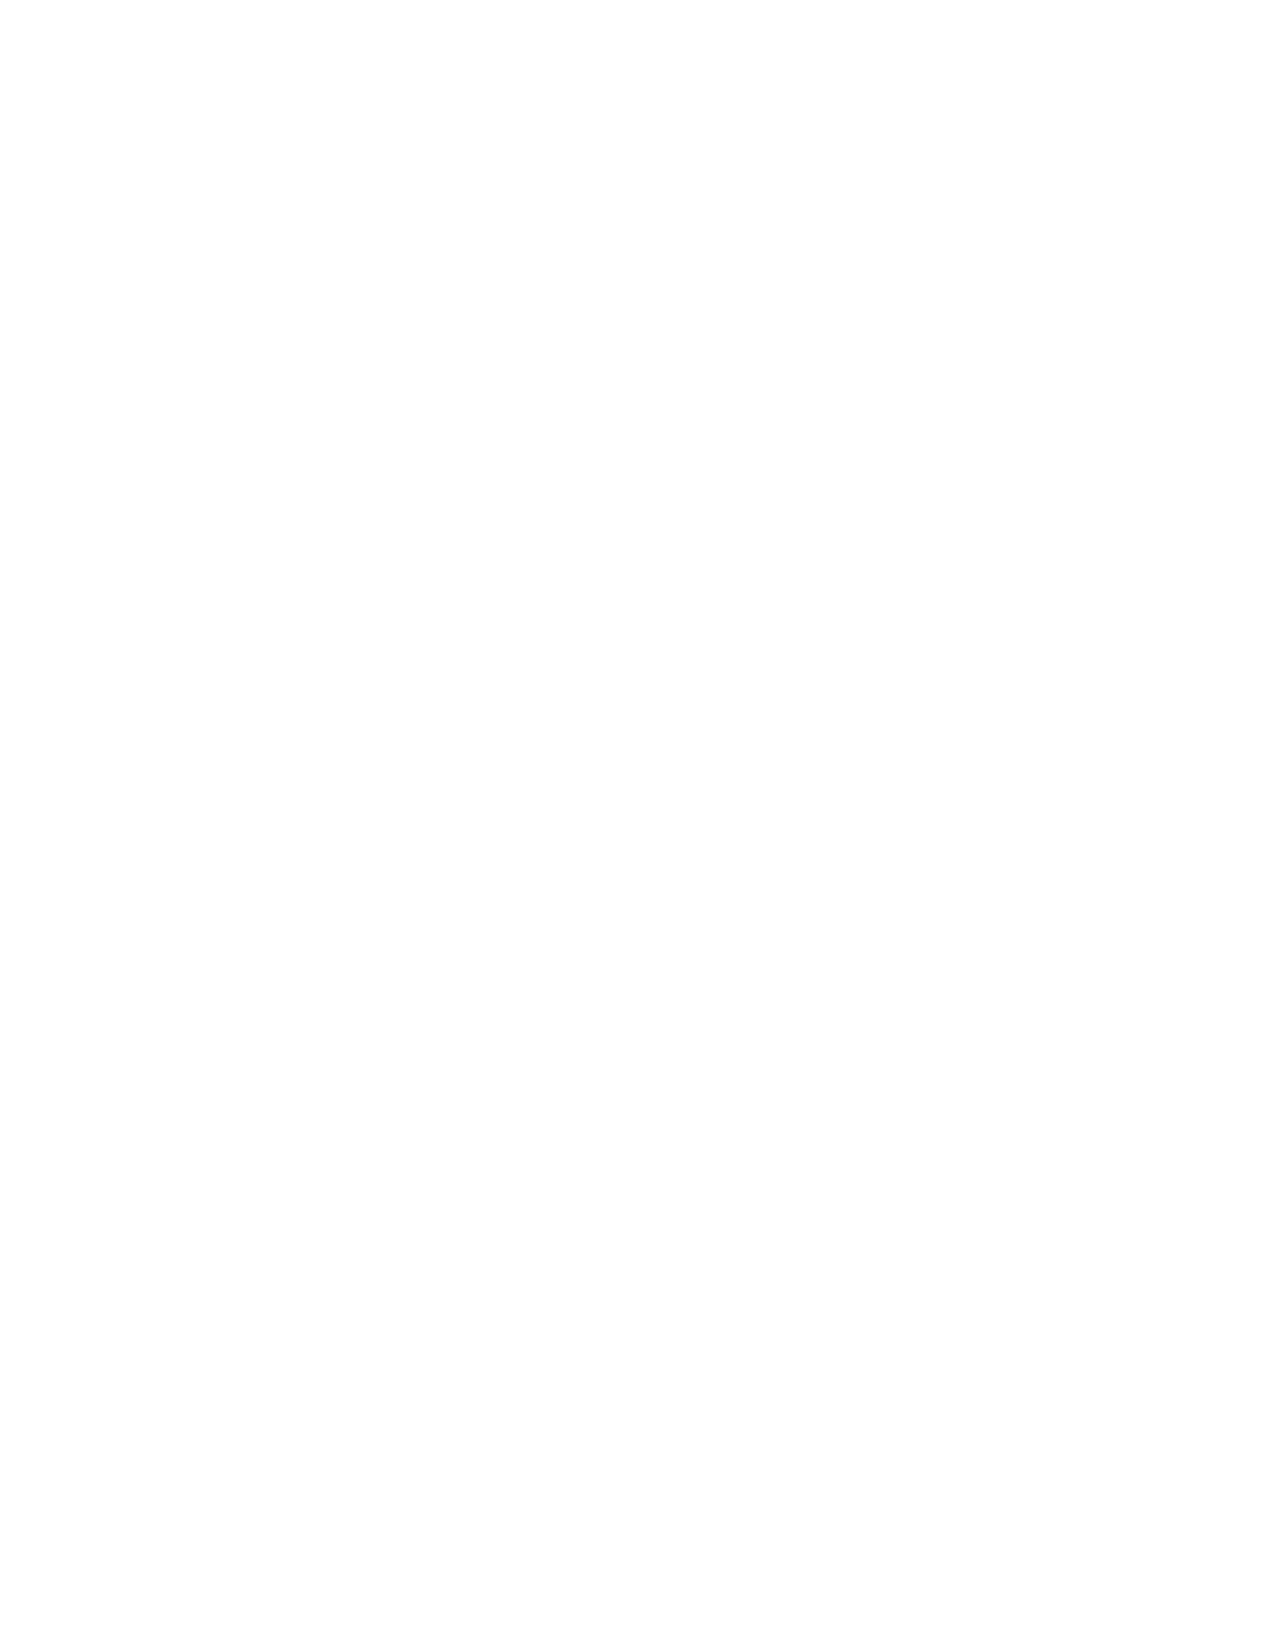
\includegraphics[max width=\textwidth]{2022_01_05_20c4aca6821d56656c19g-4}

\section{Nonlinear Models}
\subsection{Nonlinear classifiable sets}
In the section, we will extend the linearly separable sets to nonlinear case. A natural extension is like what kernel method does in SVM for binary case, we will introduce the so-called feature mapping.

Thus, we have the following natural extension for linearly separable by using feature mapping and original definition of linearly separable.

Definition 1 (nonlinearly separable sets). These data sets $A_{1}, A_{2}, \cdots, A_{k} \subset \mathbb{R}^{d}$ are called nonlinearly separable, if there exist a feature space $\mathbb{R}^{\tilde{d}}$ and a smooth (if it has derivatives of all orders) feature mapping
$$
\varphi: \mathbb{R}^{d} \mapsto \mathbb{R}^{d}
$$
such that
$$
\tilde{A}_{i}:=\varphi\left(A_{i}\right)=\left\{\tilde{x} \mid \tilde{x}=\varphi(x), x \in A_{i}\right\}, \quad i=1,2, \ldots, k
$$
are linearly separable.

Remark 1. 1. This definition is also consistent with the definition of linearly separable as we can just take $d=d$ and $\varphi=$ id if $A_{1}, A_{2}, \cdots, A_{k}$ are already linearly separable.

  \begin{enumerate}
    \setcounter{enumii}{2}
    \item The kernel method in SVM is mainly based on this idea for binary case $(\mathrm{k}=2)$ where they use kernel functions to approximate this $\varphi(x)$.

    \item For most commonly used deep learning models, they are all associated with a softmax mapping which means that we can interpret these deep learning models as the approximation for feature mapping $\varphi$.

  \end{enumerate}
However, softmax is not so crucial for this definition actually as we have the next equivalent result. Theorem 1. $A_{1}, A_{2}, \cdots, A_{k} \subset \mathbb{R}^{d}$ are nonlinearly separable is equivalent that there there exist a smooth classification function
$$
\psi: \mathbb{R}^{d} \mapsto \mathbb{R}^{k}
$$
such that for all $i=1: k$ and $j \neq i$
$$
\psi_{i}(x)>\psi_{j}(x), \quad \forall x \in A_{i}
$$
Proof. On the one hand, it is easy to see that if $A_{1}, A_{2}, \cdots, A_{k} \subset \mathbb{R}^{d}$ are nonlinearly separable then they we can just take
$$
\psi(x)=p(\varphi(x) ; \theta)
$$
where the $\boldsymbol{p}(y ; \theta)$ is the softmax function for linearly separable sets $\varphi\left(A_{i}\right)$ for $i=$ $1,2, \cdots, k$.

On the other hand, let assume that $\psi$ is the smooth classification functions for $A_{1}, A_{2}, \cdots, A_{k} \subset \mathbb{R}^{d} .$ We claim that, we can take $\varphi(x)=\psi(x)$ and then
$$
\varphi\left(A_{1}\right), \varphi\left(A_{2}\right), \cdots, \varphi\left(A_{k}\right) \subset \mathbb{R}^{k} \quad(\tilde{d}=k)
$$
will be linearly separable. Actually, if you take $\theta=(I, 0)$ in softmax mapping $\boldsymbol{p}(x ; \theta)$, then the monotonicity of $e^{x}$ show that for all $i=1: k$ and $j \neq i$
$$
\boldsymbol{p}_{i}(\varphi(x) ; \theta)=\frac{e^{\psi_{i}(x)}}{\sum_{i=1}^{k} e^{\psi_{i}(x)}}>\frac{e^{\psi_{j}(x)}}{\sum_{i=1}^{k} e^{\psi_{i}(x)}}=\boldsymbol{p}_{j}(\varphi(x) ; \theta), \quad \forall x \in A_{i} .
$$
]

Similarly to linearly separable sets, we have the next lemme for $k=2$.

Lemma 1. A $_{1}$ and $A_{2}$ are nonlinearly separable is equivalent that there exists a function $\varphi: \mathbb{R}^{d} \mapsto \mathbb{R}$ such that
$$
\varphi(x)>0 \quad \forall x \in A_{1} \quad \text { and } \quad \varphi(x)<0 \quad \forall x \in A_{2}
$$
Proof. Based the equivalence of nonlinearly separable sets, there exists $\psi_{1}(x)$ and $\psi_{2}(2)$ such that for all $i=1: 2$ and $j \neq i$
$$
\psi_{i}(x)>\psi_{j}(x), \quad \forall x \in A_{i}
$$
Then, we can just take
$$
\varphi(x)=\psi_{1}(x)-\psi_{2}(x)
$$
On the other hand, if there exist $\varphi(x)$, then we can construct $\psi_{1}(x)$ and $\psi_{2}(2)$ as
$$
\psi_{1}(x)=\frac{1}{2} \varphi(x) \quad \text { and } \quad \psi_{2}(x)=-\frac{2}{2} \varphi(x)
$$
Remark 2. Here we mention that, we only assume that for all $i=1: k$ and $j \neq i$ we have $\psi_{i}(x)>\psi_{j}(x), \forall x \in A_{i}$ for nonlinearly separable. We do not assume that $\psi_{i}(x) \geq 0$ or $\sum_{i=1}^{k} \psi_{i}(x)=1$, which means that $\psi(x)=\left(\begin{array}{c}\psi_{1}(x) \\ \psi_{2}(x) \\ \vdots \\ \psi_{k}(x)\end{array}\right)$ is not a discrete probability distribution over all k classes.

The previous theorem shows that softmax function is not so crucial in nonlinearly separable case. Combined with deep learning models, we have the following understanding about what deep learning models are approximating.

  \begin{enumerate}
    \item If a classification model is followed with a softmax, then the it is approximating the feature mapping $\varphi: \mathbb{R}^{d} \mapsto \mathbb{R}^{\bar{d}}$.

    \item If the classification model dose not followed by softmax, then it is approximating $\psi: \mathbb{R}^{d} \mapsto \mathbb{R}^{k}$ directly.

  \end{enumerate}
Example 1. Consider $k=2$ and $A_{1} \subset\left\{(x, y) \mid x^{2}+y^{2}<1\right\}, \quad A_{2} \subset\left\{(x, y) \mid x^{2}+y^{2}>1\right\}$, then we can have the following nonlinear feature mapping:

\includegraphics[max width=\textwidth]{2022_01_05_20c4aca6821d56656c19g-7}

Here we have the following comparison for linear and nonlinear models from the viewpoint of loss functions:

Linear case (Logistic regression):
$$
L_{\lambda}(\theta)=\sum_{j=1}^{N} \ell\left(y_{j}, p\left(x_{j} ; \theta\right)\right)+\lambda R(\|\theta\|)
$$
Nonlinear case:
$$
L_{\lambda}(\theta)=\sum_{j=1}^{N} \ell\left(y_{j}, p\left(\varphi\left(x_{j} ; \theta_{1}\right) ; \theta_{2}\right)\right)+\lambda R(\|\theta\|)
$$
Remark 3. We have the following remarks.
$$
\text { 1. } \ell(q, p)=\sum_{i=1}^{k}-q_{i} \log p_{i} \leftrightarrow \text { cross-entropy }
$$

  \begin{enumerate}
    \setcounter{enumii}{2}
    \item $p(x ; \theta)=\operatorname{softmax}(W x+b)$ where $\theta=(W, b)$

    \item $\theta=\left(\theta_{1}, \theta_{2}\right)$ for nonlinear case

    \item $\lambda R(\|\theta\|) \leftrightarrow$ regularization term

  \end{enumerate}
In general, we have the following popular nonlinear models for $\varphi(x ; \theta)$

  \begin{enumerate}
    \item Polynomials.

    \item Piecewise polynomials (finite element method).

    \item Kernel functions in SVM.

    \item Deep neural networks.

  \end{enumerate}
\section{References}
[1] L. Chen, P. Sun, and J. Xu. Optimal anisotropic meshes for minimizing interpolation errors in $l^{p}$-norm. Mathematics of Computation, $76(257): 179-204,2007 .$

[2] K. He, X. Zhang, S. Ren, and J. Sun. Deep residual learning for image recognition. In Proceedings of the IEEE Conference on Computer Vision and Pattern Recognition, pages 770-778, 2016

[3] K. He, X. Zhang, S. Ren, and J. Sun. Identity mappings in deep residual networks. In European Conference on Computer Vision, pages 630-645. Springer, $2016 .$

[4] M. Leshno, V.Y. Lin, A. Pinkus, and S. Schocken. Multilayer feedforward networks with a nonpolynomial activation function can approximate any function. Neural networks, 6(6):861-867, 1993 .

[5] A. Pinkus. Approximation theory of the mlp model in neural networks. Acta numerica, $8: 143-195,1999 .$

[6] L. R. Scott and S. Zhang. Finite element interpolation of nonsmooth functions satisfying boundary conditions. Mathematics of Computation, $54(190): 483-493$, $1990 .$

[7] J. Xu. Finite element methods. Lecture notes, 2020 .


\end{document}